\documentclass[conference, onecolumn]{IEEEtran}
\IEEEoverridecommandlockouts
\usepackage{cite}
\usepackage{amsmath,amssymb,amsfonts}
\usepackage{algorithmic}
\usepackage{graphicx}
\usepackage{textcomp}
\usepackage{xcolor}
\usepackage{flushend}
\def\BibTeX{{\rm B\kern-.05em{\sc i\kern-.025em b}\kern-.08em
    T\kern-.1667em\lower.7ex\hbox{E}\kern-.125emX}}
\begin{document}

\title{SU 2024 IOT102 Project Title\\
}

\author{
1\textsuperscript{st} Student Name, 2\textsuperscript{nd} Student Name, 3\textsuperscript{rd} Student Name,\\ 4\textsuperscript{th} Student Name, and Duc Ngoc Minh Dang\\
FPT University, Ho Chi Minh Campus, Vietnam\\
\{Student1, Student2, Student3, Student4\}@fpt.edu.vn, and ducdnm2@fe.edu.vn}
\maketitle

\begin{abstract}
Put the abstract here.
\end{abstract}

\section{Introduction}
Give the \textcolor{red}{overview} of research problems (domestic and overseas).

\begin{figure}[htbp]
\centerline{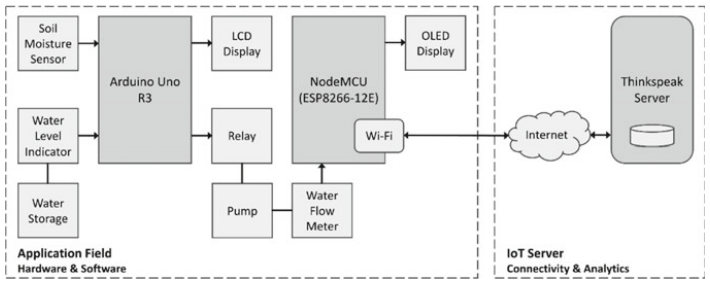
\includegraphics[width=4.8 in]{Block_diagram.png}}
\caption{Block diagram of the developed system.}
\label{fig}
\end{figure}

\section{Main proposal}
Necessity and topicality, \emph{the scientific and practical} significance of the research topic.\\

\subsection{System models and block diagram}

\subsection{Components and peripheral devices}

\subsection{Software programming}

\subsection{Programming Flowchart}

\section{Results and discussion}
A clear concise description of the research methods used.\\

\subsection{Prototype Implementation}
Cite here \cite{Tellez_2016}

\subsection{Experimental Results}

\subsection{Discussion}


\section{Conclusion}
Give a clear concise description of the project’s outputs \cite{Li_2018} \\

\emph{This is an example of a citation.}
For papers published in translation journals, please give the English citation first, followed by the original foreign-language citation \cite{dang2014her,anh2020waste,Khorov_2018,dang2015hybrid}  \cite{pham_jit}.

\section{Author's contribution}

\begin{table}
    \centering
\caption{Author's contribution}
\label{tab:my_label}
    \begin{tabular}{|c|c|c|c|c|}
    \hline
         \#&  Student ID &  Student Name &  Tasks & Contribution\\
         \hline
         1&  SE181235&  Nguyen Van A&  Draw block diagram, flowchart& 25\%\\
         \hline
         2&  &  &  Study conception and design& 30\%\\
         \hline
         3&  &  &  Program Arduino and ESP8266& 25\%\\
         \hline
         4&  &  &  Write report, prepare Presentation & 20\%\\
         \hline
         \multicolumn{4}{|c|}{Total}& 100\%\\
         \hline
    \end{tabular}    
\end{table}

\bibliographystyle{IEEEtran}  %use this for IT
\bibliography{Bib_references}
\end{document}